\begin{slide}{８．４　陰関数と条件下の極値}
\begin{itemize}
\item 陰関数(implicit function)とは$f(x,y) = 0$のように書かれる関数を指す。
\item 陽関数(explicit function)とは$z = g(x,y)$のように従属変数が独立変数で明示的に表される関数を指す。
\item 関数の極値は微分や偏微分で求めるが、変数に制約条件(constraint)がある場合には、ラグランジュ乗数\footnote{ラグランジュ未定乗数という訳もあり}(Lagrange multiplier)を用いて解く。
\end{itemize}
\end{slide}
\begin{slide}{制約条件下での極値の例}
\begin{equation}
f(x,y) = x^2 - y^2 + 3 \nonumber
\end{equation}
の極値を
\begin{equation}
g(x, y) = 1 - x^2 - y^2 = 0\nonumber
\end{equation} 
の制約条件（$x, y$が半径１の円周上を動く)下で$f(x,y) = x^2 - y^2 +3$の極大・極小を求める。
\begin{figure}[h]
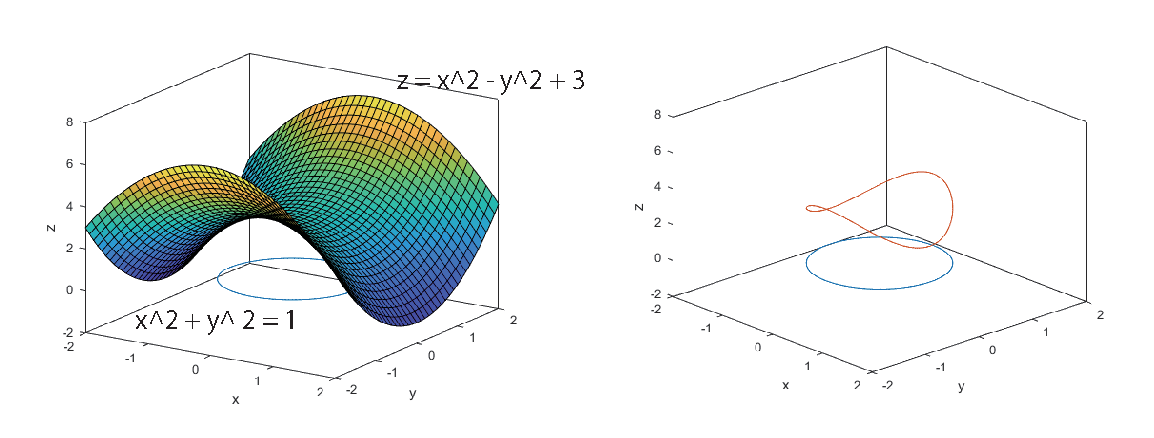
\includegraphics[width=8cm]{calculus13/lag.eps}
\end{figure}
\end{slide}
\begin{slide}{ラグランジュ乗数による解}
拘束条件にラグランジュ乗数$\lambda$を掛け、極値問題を拡大(augment). 
\begin{equation}
f_a(x,y) = f(x,y) + \lambda g(x,y) \nonumber
\end{equation}
$x,y$に関して偏微分してそれを０とする$x,y$を求める。
\begin{eqnarray}
\frac{\partial f_a}{\partial x} &=& \frac{\partial f}{\partial x} + \lambda \frac{\partial g}{\partial x} = 0 \nonumber \\
\frac{\partial f_a}{\partial y} &=&\frac{\partial f}{\partial y} + \lambda \frac{\partial g}{\partial y} = 0 \nonumber 
\end{eqnarray}
$f(x,y)=x^2-y^2+3, g(x) = 1-x^2-y^2$に適用すると
\begin{eqnarray}
&& 2x - \lambda(2x) = 0 \label{eq:lag1}  \\
&&-2y  - \lambda(2y) = 0 \label{eq:lag2}
\end{eqnarray}
\pref{eq:lag1}に$y$, \pref{eq:lag2}に$x$を掛けて引いて$\lambda$を消去すると$xy=0$となる。拘束条件を考慮すると($x=0, y=\pm 1$)あるいは( $y=0, x=\pm 1$)が極値を与える。
\end{slide}
\begin{slide}{ラグランジュ乗数による解2}
\begin{itemize}
\item $f(x,y) = x^2 - y^2 + 3$から$f_{xx} = 2, f_{yy} = -2, f_{xy} =0$、ヘシアン$\Delta = f_{xx}f_{yy} - f_{xy}^2<0$なので、制約条件がなければ極値は取らない
\item 制約条件$g(x,y)$がある場合には、変化できる方向が限定されているので、極値が存在。
\item $x=0, y=\pm 1$の場合には$x$方向しか動けないので$f_{xx}=2$のみが有効で極小、 $y=0, x=\pm 1$は$y$方向しか動けないので極大。
\item 極大・極小はグラフの形からも判断することもできる。
\end{itemize}
\end{slide}
\begin{slide}{ラグランジュ乗数補足(参考)}
極値では傾きがゼロになるので、$x,y$が$x+dx, y+dy$に移動しても値は同じ
\begin{equation}
f(x+dx, y+dy) = f(x, y) + f_x(x,y) dx + f_y(x,y) dy  =f(x,y) \label{eq:lagd}
\end{equation}
となり$f_x(x,y) dx + f_y(x,y) dy = 0$である。一方、拘束条件は移動後の$x+dx, y+dy$でも満足されないといけないので
\begin{equation}
g(x+dx, y+dy) = g(x,y) + g_x(x,y)dx + g_y(x,y) dy = 0 \nonumber
\end{equation}
$g(x,y)=0$なので
\begin{equation}
dy = -\frac{g_x}{g_y} dx \nonumber 
\end{equation}
\pref{eq:lagd}に代入して
\begin{equation}
f_x dx -f_y \frac{g_x}{g_y} dx= (f_x - \frac{f_y}{g_y} g_x)dx \label{eq:lagd2}
\end{equation}
\end{slide}
\begin{slide}{ラグランジュ乗数補足2}

\pref{eq:lagd2}がどのような$dx$に対しても成立するためには
\begin{equation}
f_x - \frac{f_y}{g_y} g_x = 0 \label{eq:lagf1}
\end{equation}
同様にどのような$dy$に対しても以下の式が成立する必要がある。
\begin{equation}
f_y - \frac{f_x}{g_x}g_y = 0 \label{eq:lagf2}
\end{equation}
どちらも変形すると
\begin{equation}
\frac{f_y}{g_y} = \frac{f_x}{g_x} = -\lambda \label{eq:lm}
\end{equation}
となり、この比の符号を反転してラグランジュ乗数として用いる。

\pref{eq:lm}を用いると\pref{eq:lagf1}, \pref{eq:lagf2}は
\begin{eqnarray}
f_x +\lambda g_x &=& 0 \nonumber \\
f_y +\lambda g_y &=& 0 \nonumber 
\end{eqnarray}
この式は$f_a = f + \lambda g$を偏微分して得られる。
\end{slide}
\begin{slide}{ラグランジュ乗数を用いない解法}
パラメタ$\theta, \quad 0 \leqq \theta < 2\pi$を用いると拘束条件$g(x)=1-x^2-y^2 =0$を用いて
$x = \cos\theta, y= \sin\theta$であり、関数は
$f=x^2 - y^2 + 3 = \cos^2\theta - \sin^2\theta + 3 = 2\cos^2\theta +2 $と一変数関数に変換できる。
極値を微分で求める
\begin{equation}
\frac{df}{d\theta} = -4\cos\theta\sin\theta  = -2\sin{(2\theta)} \nonumber
\end{equation}
なので、$\theta=0, \frac{\pi}{2}, \pi, \frac{3\pi}{2}$で$\frac{df}{d\theta}=0$となり極値である。対応する$(x,y)$はそれぞれ$(1,0), (0,1), (-1,0), (0,-1)$
\begin{figure}[h]
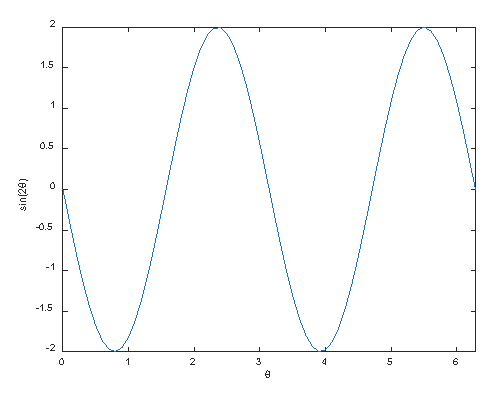
\includegraphics[width=3cm]{calculus13/paralag.eps}
\end{figure}
また$\frac{d^2f}{d\theta^2}=-4\cos(2\theta)$なので、極値は順に極大、極小、極大、極小である。

\end{slide}
\begin{slide}{問題８．６(1)}
\begin{itemize}
\item $x^2 + 4y^2 - 4 = 0$の条件下で$f(x,y)=xy$の極値を求めよ
\begin{figure}[h]
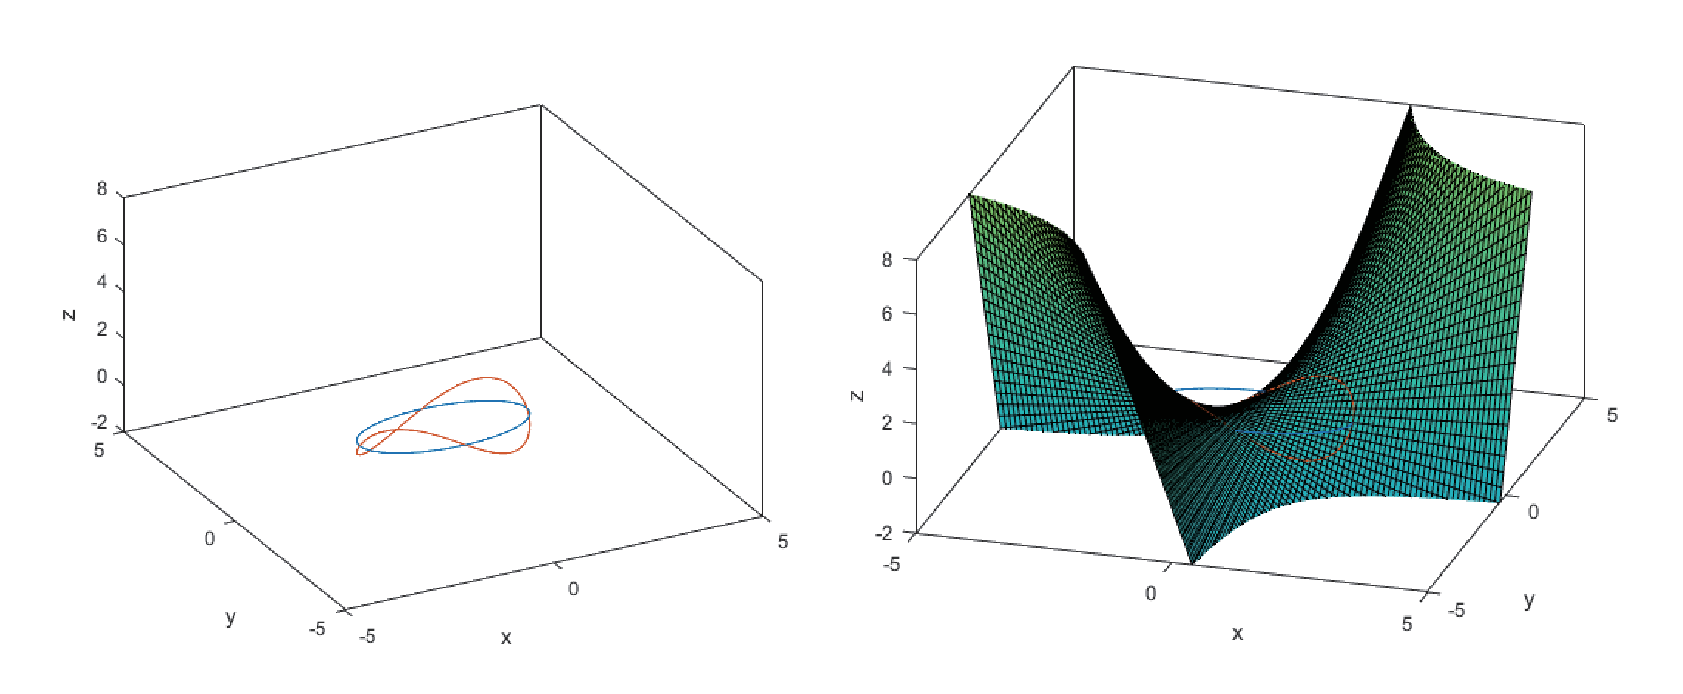
\includegraphics[width=6cm]{calculus13/lag2.eps}
\end{figure}
$x,y$が同符号の時は$xy$の絶対値に単調増加、異符号の時は$xy$の絶対値に単調減少。
\end{itemize}
\end{slide}
\begin{slide}{問題８．６（２）}
\begin{itemize}
\item $x^2+y^2 -1 = 0$の条件下で$f(x,y)=2x+3y$の極値を求めよ。
\end{itemize}
\begin{figure}[h]
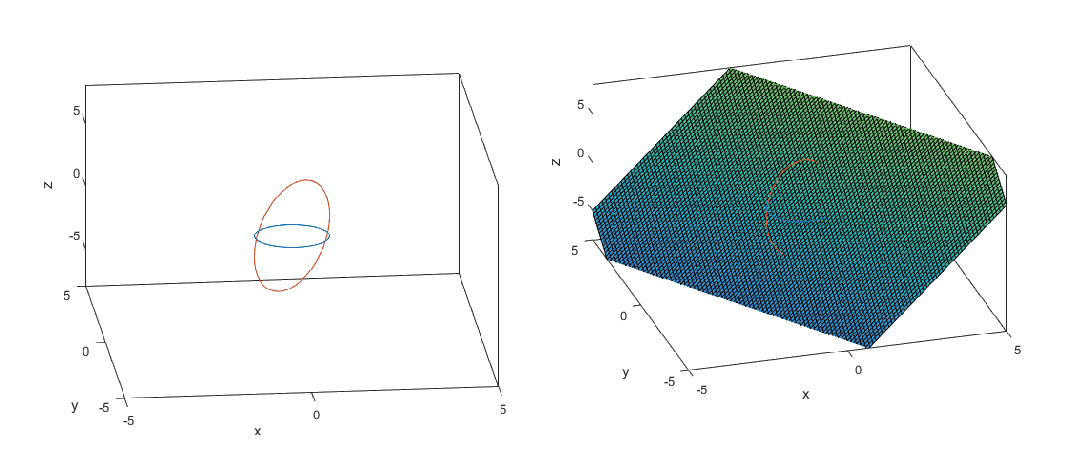
\includegraphics[width=6cm]{calculus13/lag3.eps}
\end{figure}
$f(x,y)$は平面
\end{slide}
\begin{slide}{９　重積分(multiple integral)}
\begin{itemize}
\item これまでは変数が一つの場合の積分を扱ってきた。$\int_a^b f(x)dx$は$a\leqq x \leqq b$の範囲の$f(x)$の面積や曲線の長さを求めることである\footnote{断面積がわかれば体積が求められる}
\item 変数が二つの関数$z=g(x,y)$を$a \leqq x \leqq b$と$c \leqq y \leqq d$の範囲で重積分すると$g(x,y)$の体積や表面積が求められる。
\end{itemize}
\begin{figure}[h]
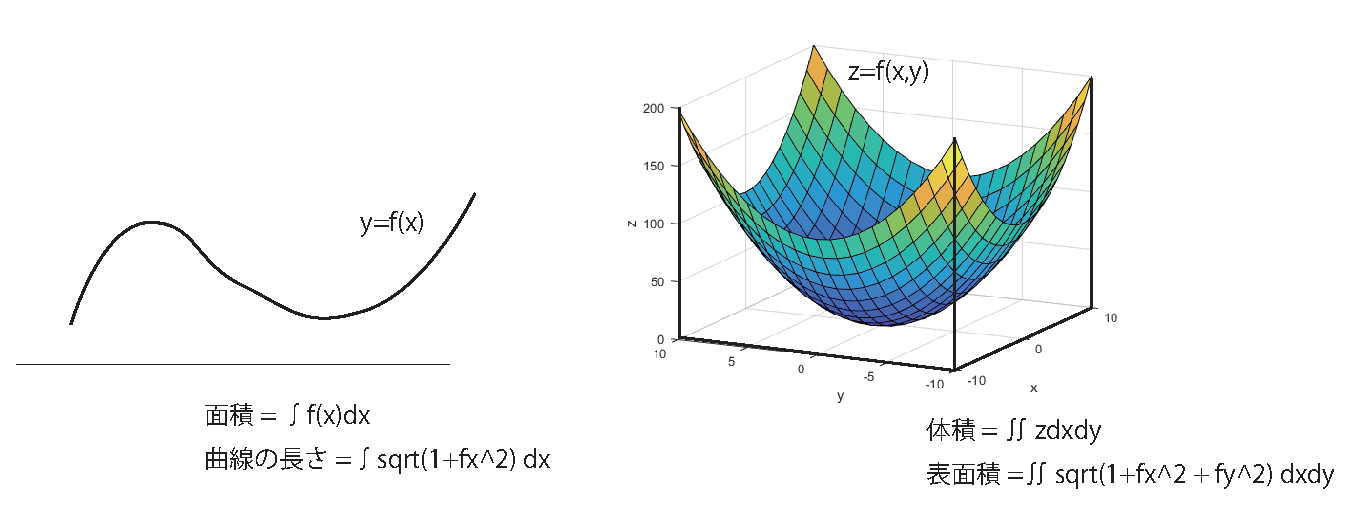
\includegraphics[width=10cm]{calculus13/paraint.eps}
\end{figure}
\end{slide}

\begin{slide}{定理９．１}
\begin{itemize}
\item 関数$f(x,y)$が$A=\left\{x,y | a \leqq x \leqq b \quad c \leqq y \leqq d\right\}$で連続ならば
$f(x,y)$は$A$で重積分可能で、定積分を繰り返すこと（累次積分 iterated integral）に置き換えられる。
\item 累次積分では$dx dy$の順序と積分範囲の指定が入れ子になるように注意。
\begin{equation}
\iint_A f(x,y) dx dy = \int_c^d \int_a^b f(x,y) dx dy = \int_a^b\int_c^d f(x,y) dy dx \nonumber
\end{equation}
\end{itemize}
\end{slide}
\begin{frame}[fragile]{例題９．１}
積分せよ
\begin{equation}
I = \iint xy dxdy, \quad A=\left\{x,y | 0\leqq x \leqq 1 \quad 0\leqq y \leqq 2\right\} \nonumber
\end{equation}

解答例
\begin{equation}
\iint_A xy dxdy = \int_0^2 \left[\frac{1}{2}x^2y\right]_0^1 dy = \int_0^2 \frac{1}{2}y dy = \left[\frac{1}{4}y^2\right]_0^2 = 1 \nonumber
\end{equation}
累次積分が逆でも答えは同じ
\begin{equation}
\iint xy dxdy = \int_0^1 \left[\frac{1}{2}xy^2\right]_0^2 dx = \int_0^1 2x dy = \left[x^2\right]_0^1 = 1 \nonumber
\end{equation}
\end{frame}
\begin{slide}{問題９．１}
重積分せよ
\begin{itemize}
\item 
\begin{equation}
I = \iint_A x dxdy, \quad A=\left\{x,y | 1\leqq x \leqq 2 \quad 0\leqq y \leqq 1\right\} \nonumber
\end{equation}
\item 
\begin{equation}
I = \iint_A \sin{x}\cos{y} dxdy, \quad A=\left\{x,y | 0\leqq x \leqq \pi  \quad 0\leqq y \leqq \frac{\pi}{2} \right\} \nonumber
\end{equation}

\end{itemize}
\end{slide}
\begin{slide}{定理９．２}
\begin{itemize}
\item 領域$D$が連続関数$\phi(x), \psi(x)$を用いて$D=\left\{x,y | \phi(x) \leqq y \leqq \psi(x)  \quad \alpha \leqq x \leqq \beta\right\}$と表されるなら、$D$の連続関数$f(x,y)$は重積分可能である。
\begin{equation}
\iint_D f(x,y) dx dy = \int_\alpha^\beta \int_{\phi(x)}^{\psi(x)}  f(x,y) dy dx \nonumber
\end{equation}
\item 領域$D$が連続関数$\phi(y), \psi(y)$を用いて$D=\left\{x,y | \phi(y) \leqq x \leqq \psi(y)  \quad \alpha \leqq y \leqq \beta\right\}$と表されるなら、$D$の連続関数$f(x,y)$は重積分可能である。
\begin{equation}
\iint_D f(x,y) dx dy = \int_\alpha^\beta \int_{\phi(y)}^{\psi(y)}  f(x,y) dx dy\nonumber
\end{equation}
\item 領域$D$で積分する場合には、$D$の領域を図示などで確認することが大事である。
\end{itemize}
\end{slide}
\begin{slide}{例題９．２}
\begin{equation}
\iint_D x^2y dx dy, \qquad  D: x^2+ y^2 \leqq 2x, \quad y \geqq 0  \nonumber
\end{equation}
 解答例:領域$D$は
\begin{equation}
(x - 1)^2 + y^2 \leqq 1 \quad y \geqq 0 \nonumber
\end{equation}
と書き換えられるので、以下の半円である。
\begin{figure}[h]
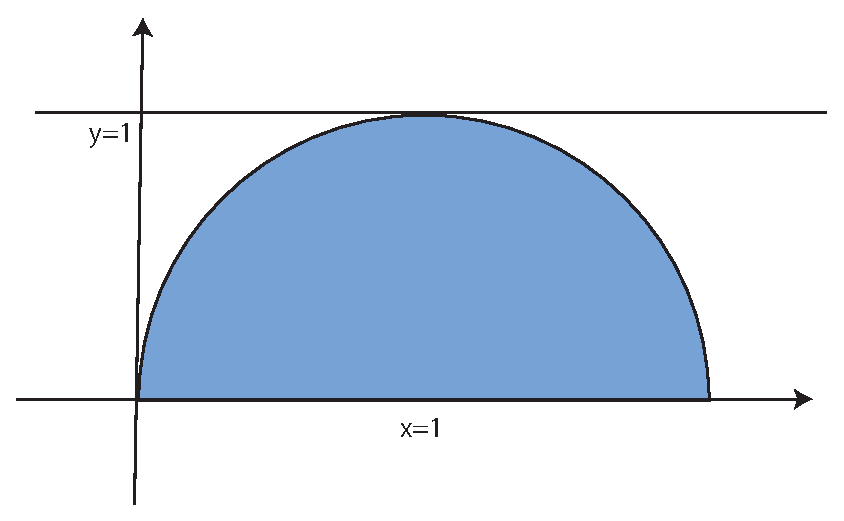
\includegraphics[width=2.5cm]{calculus13/iint.eps}
\end{figure}
\begin{eqnarray}
\iint_D x^2 ydx dy &=& \int_0^2 \int_0^{\sqrt{2x-x^2}} x^2y dy dx = \int_0^2 \left[\frac{1}{2}x^2y^2\right]_0^{\sqrt{2x-x^2}} dx \nonumber \\
&=& \int_0^2 \frac{1}{2}x^2(2x-x^2) dx = \frac{4}{5} \nonumber 
\end{eqnarray}
\end{slide}
\begin{slide}{問題９．２　重積分せよ}
\begin{enumerate}
\item 
\begin{equation}
\iint_D x dx dy, \qquad  D: x+y \leqq 1, x \geqq 0, y\geqq 0 \nonumber
\end{equation}
\item 
\begin{equation}
\iint_D xy dx dy, \qquad  D: x\leqq y \leqq 2-x, x \geqq 0 \nonumber
\end{equation}
\end{enumerate}
\end{slide}
\begin{slide}{7/21(月）は授業内テスト}
\begin{itemize}
\item 時間は70 分(予定）。
\item 資料持ち込み可能。ネットで調べてもよいが、質問して答えやヒントをもらってはいけない。Chat GPTなどのLLMも禁止。
\item 表計算ソフトを使う、プログラムを書くなどしてコンピュータで答えを求めてもよい。
\item 学生証を机の上に出す。
\item テストが何等かの事情で受けられない場合には、7月17日(木）までにKLMSで申し出ること。当日、急病・事故などの場合には、無理せず事後でもよいので、7/23（水）までに連絡してください。数が確定次第、別手段を考えます。例年だと面談です。
\end{itemize}
\end{slide}